\documentclass{article}
\usepackage[utf8]{inputenc}
\usepackage{graphicx}
\title{TUGAS DATABASE 2}
\author{John Kevin Giraldi (1184049) }
\date{1 November 2019}

\begin{document}

\maketitle

\par
Cara membuat Aplikasi pada Oracle APEX
\begin{enumerate}
    \item Pertana kita harus melakukan Login untuk mengakses web Oracle Apex tersebut.
    \begin{figure}[h]
	\centering
	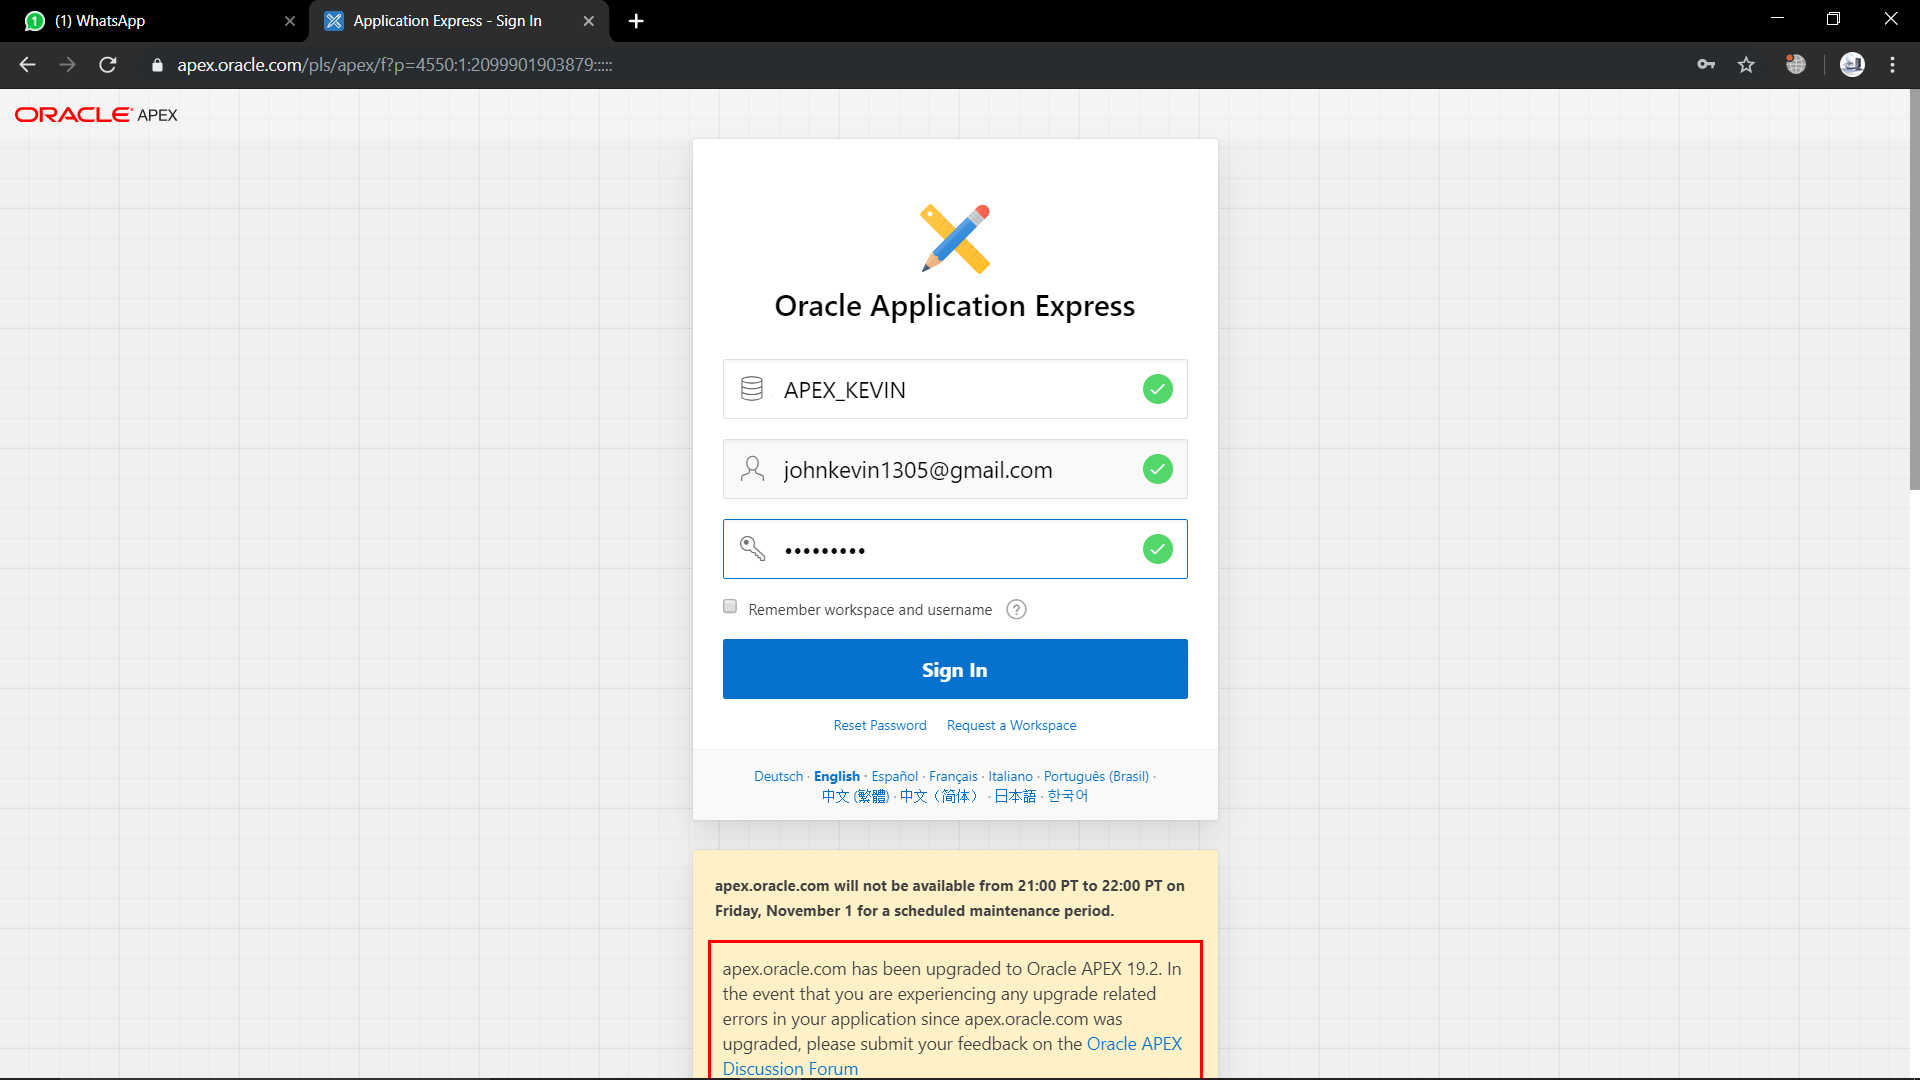
\includegraphics[width=8cm]{Figure/Login.png}
	\caption{Login}
	\label{fig:gambar}
	\end{figure}

    \item Selanjutnya pilih "App Builder" lalu klik "Create"
    \begin{figure}[h]
	\centering
	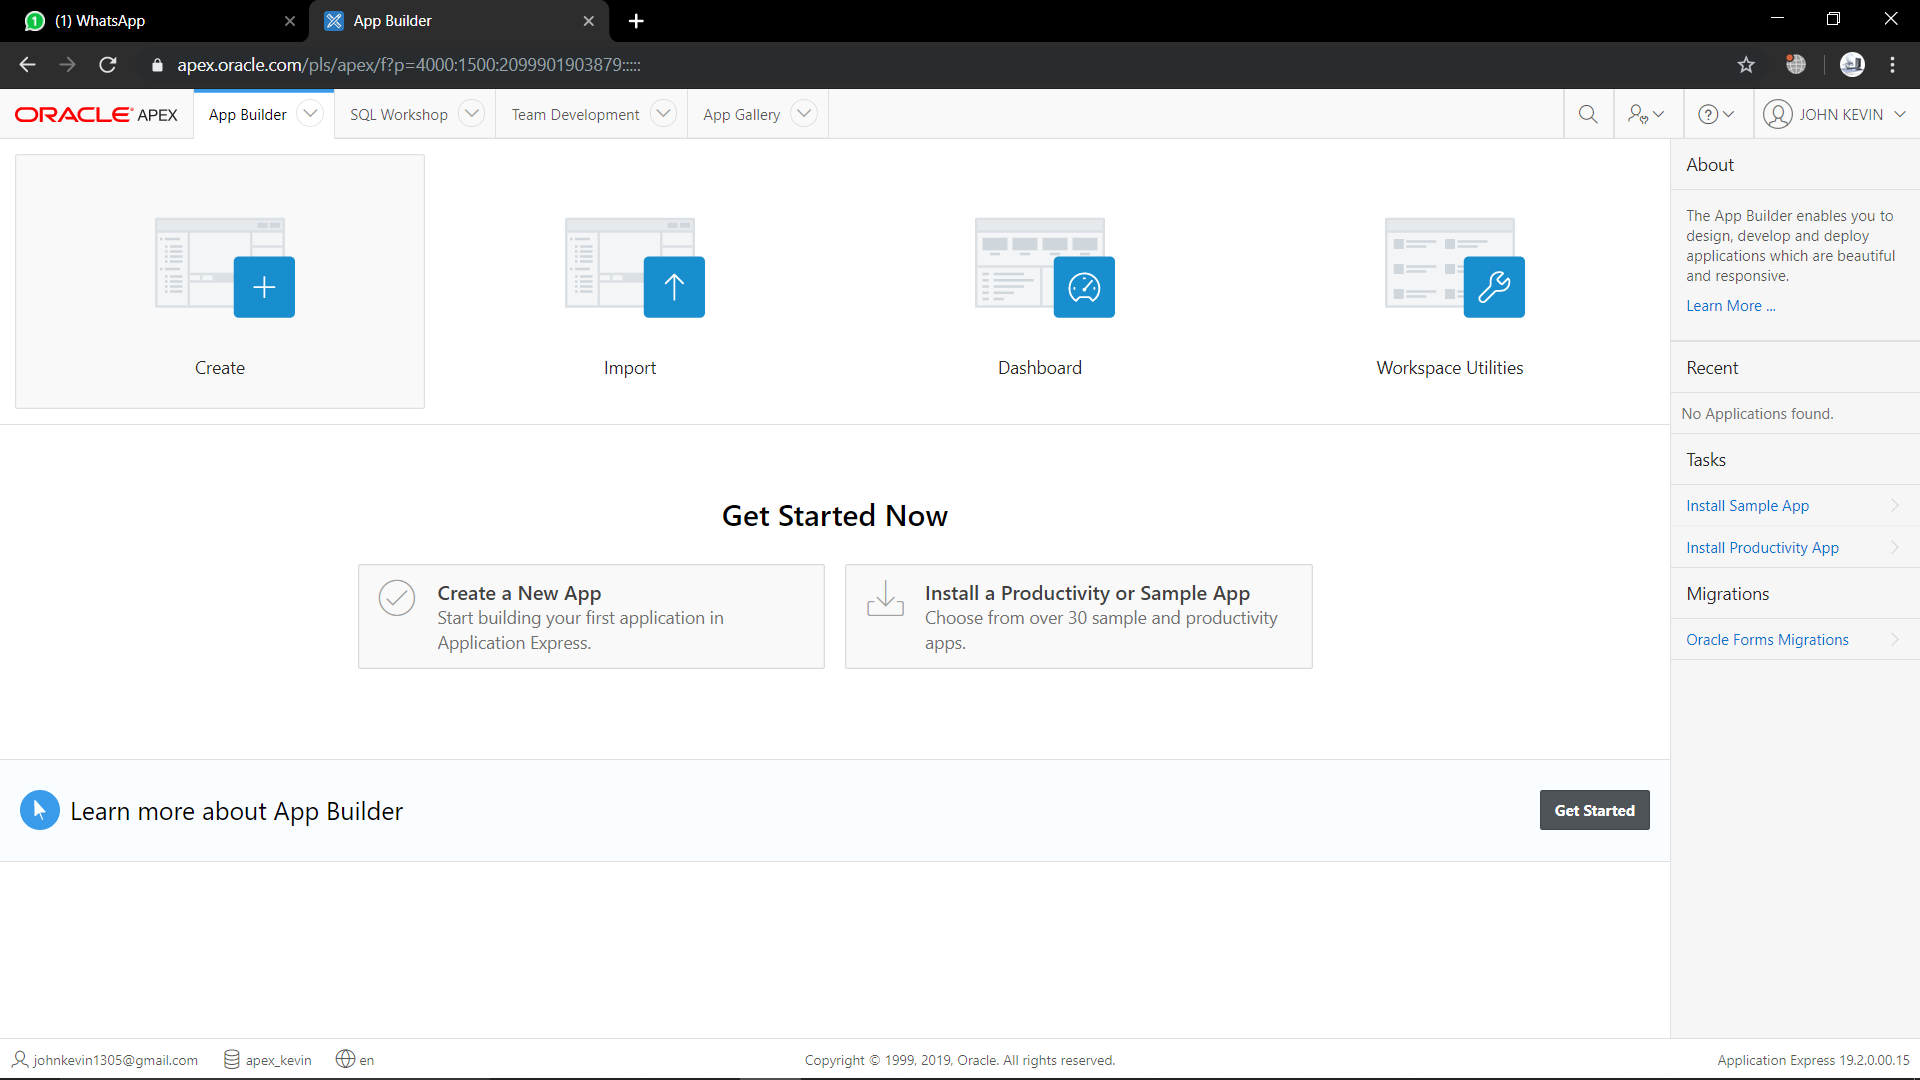
\includegraphics[width=8cm]{Figure/Create.png}
	\caption{Create}
	\label{fig:gambar}
	\end{figure}

    \item Setelah itu kalian klik "From a File"
    \begin{figure}[h]
	\centering
	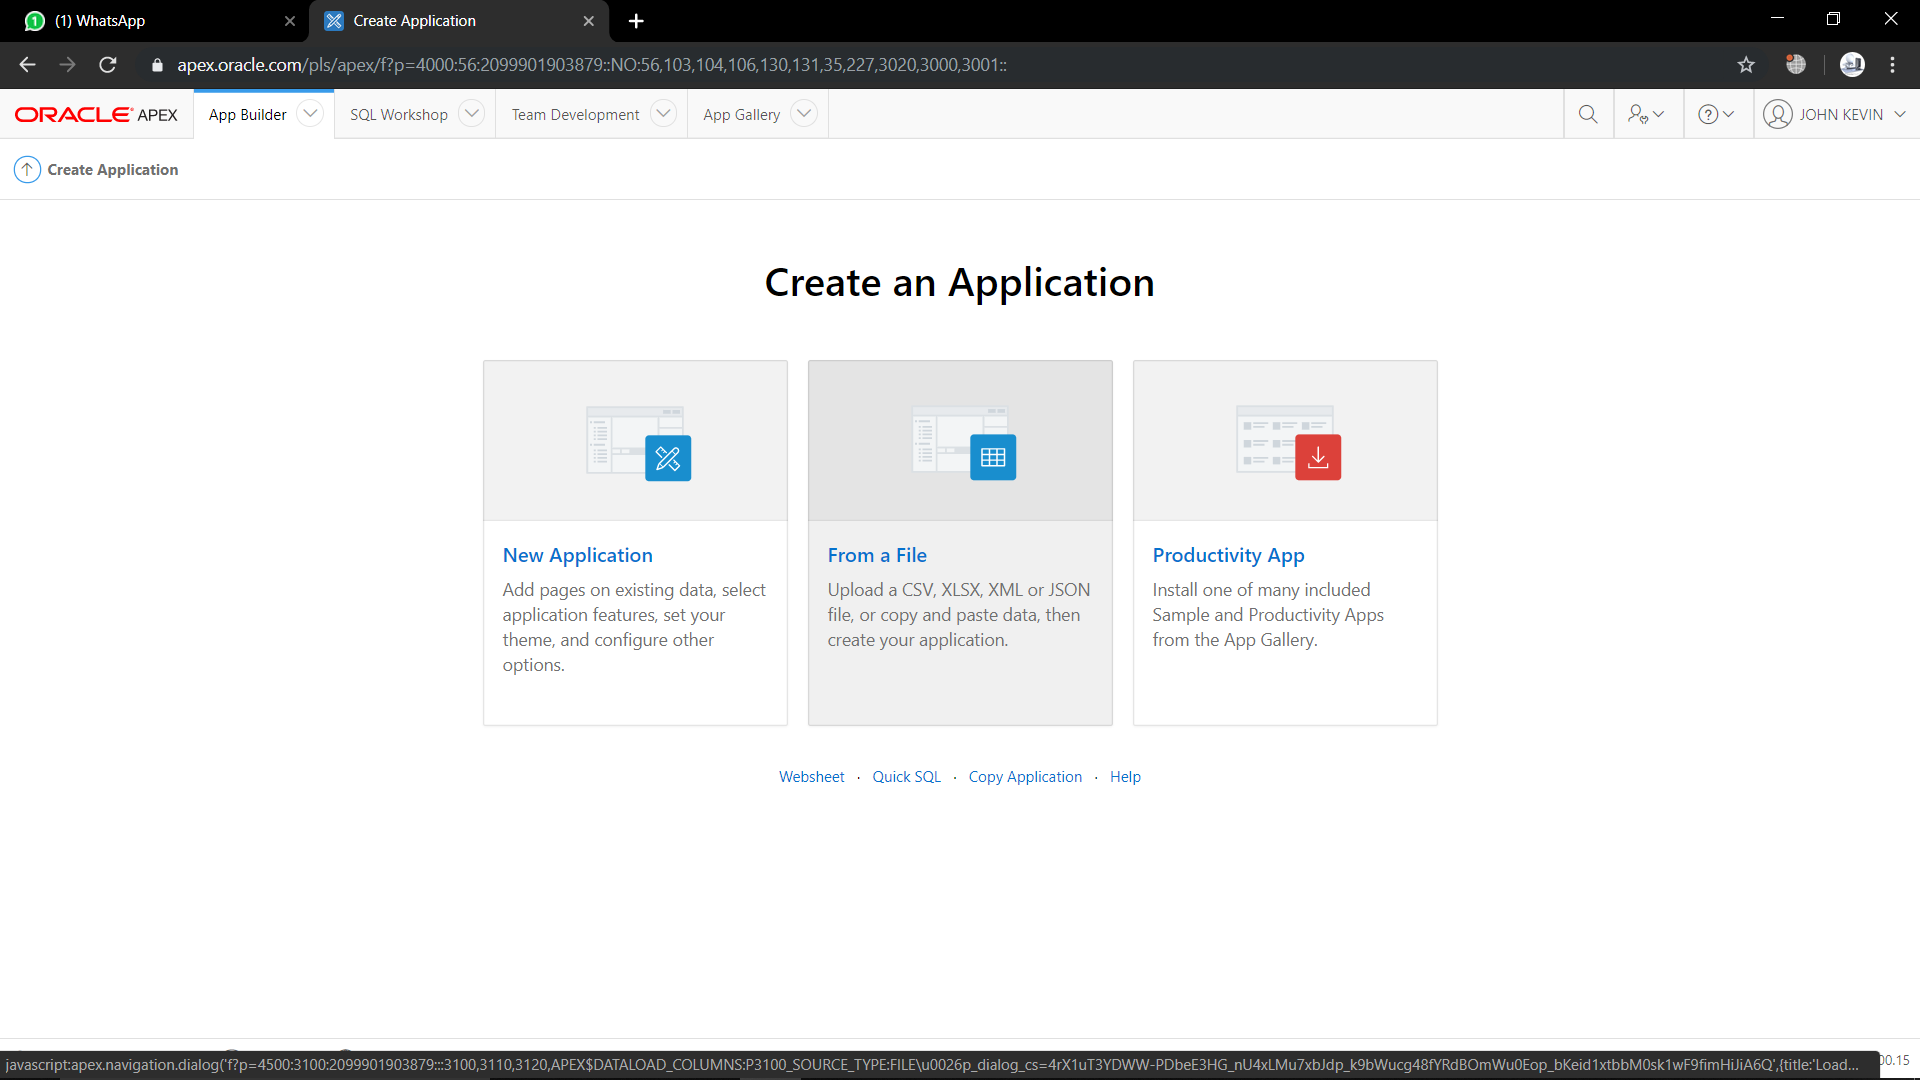
\includegraphics[width=6cm]{Figure/FOF.png}
	\caption{From a File}
	\label{fig:gambar}
	\end{figure}

    \item Masukkan file yang akan kalian buat, ada dua cara yang dapat anda lakukan, cara yang pertama dengan "Upload File". Cara yang kedua "Copy and Paste". Saya disini dengan cara "Upload File" file yang akan dibuat.
     \begin{figure}[!htbp]
        \centering
        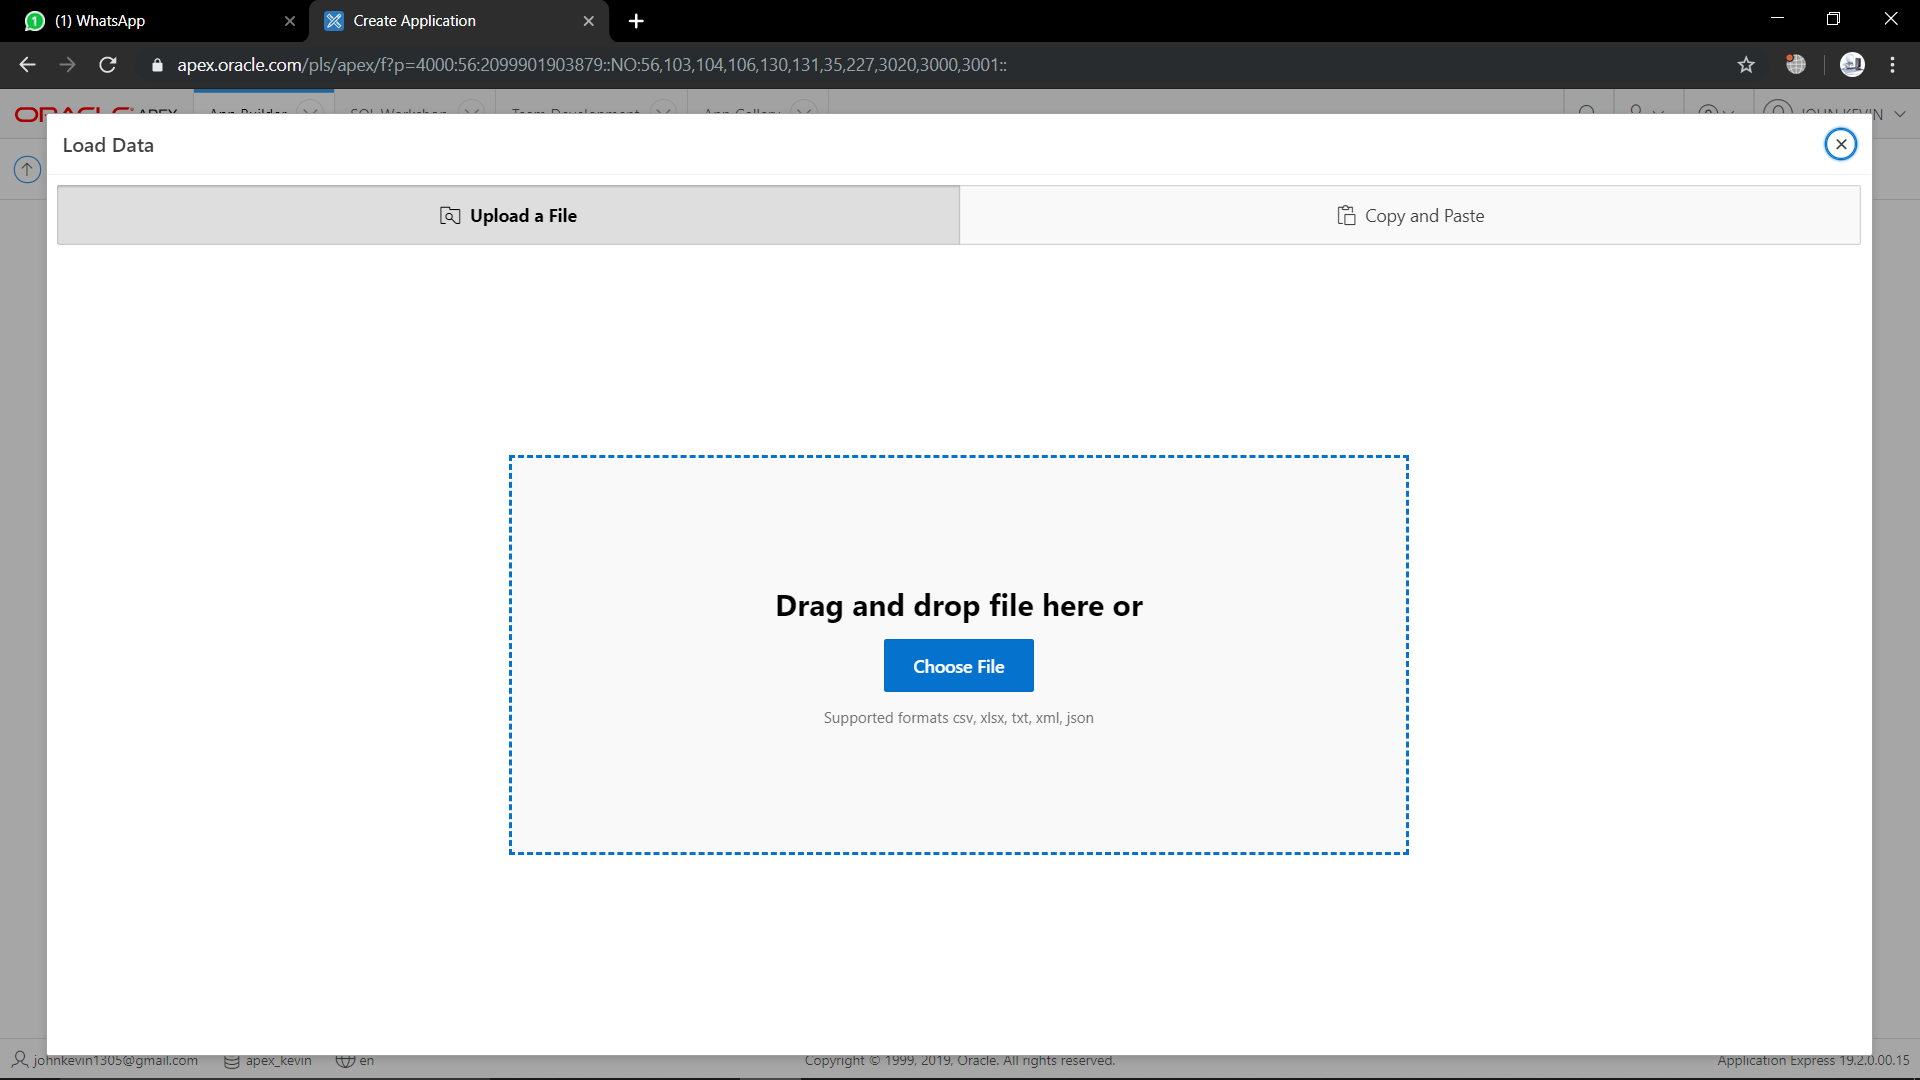
\includegraphics [width=6cm]{Figure/CF.png}
        \caption{Caption}
        \label{capture3}
    \end{figure}
    
    \item Isi "Table Name" yang kalian inginkan, untuk eror tabel name atau "Table Name Error" akan otomatis terisi. Jika sudah lalu klik "Load Data"
    \begin{figure}[h]
	\centering
	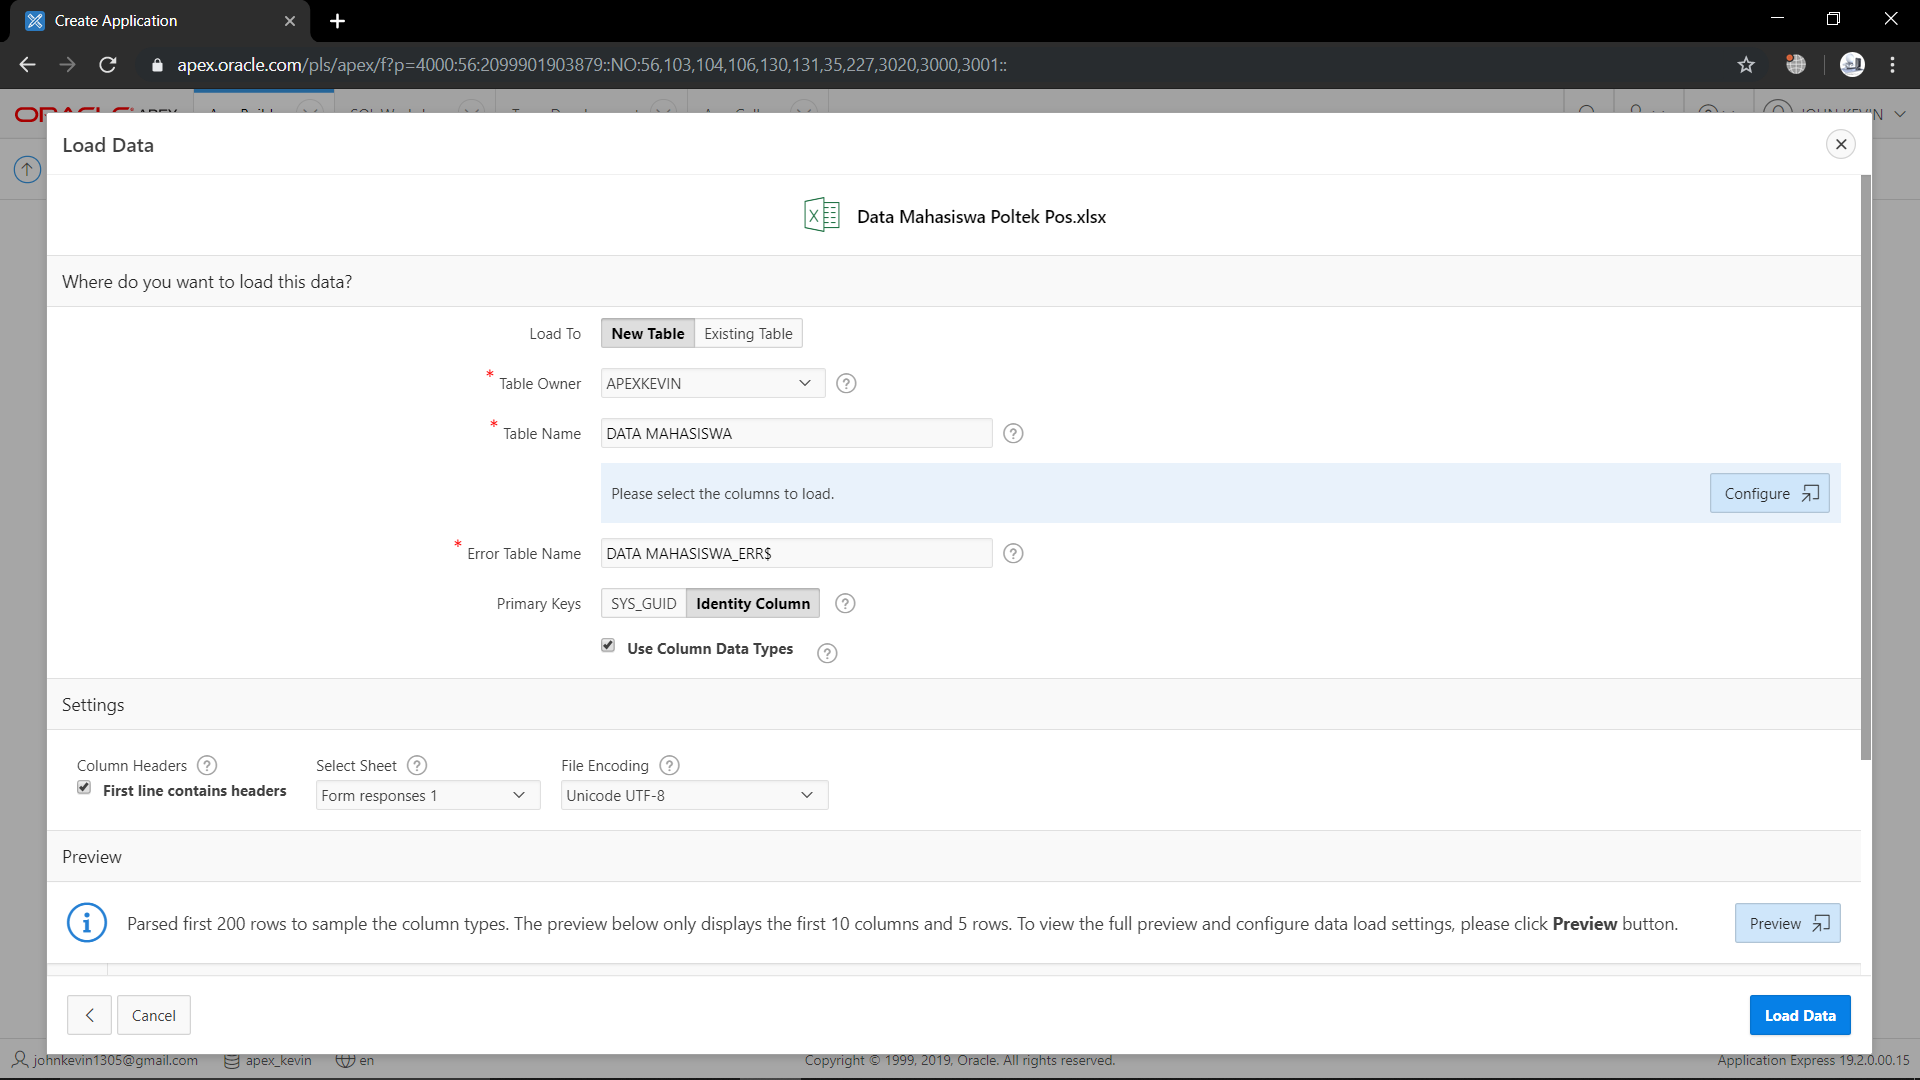
\includegraphics[width=7cm]{Figure/ID.png}
	\caption{Create}
	\label{fig:gambar}
	\end{figure}
	
    \item Jika berhasil pada tahap "Load Data" tadi, maka akan ada ceklis hijau lalu klik "View Table"
    \begin{figure}[h]
	\centering
	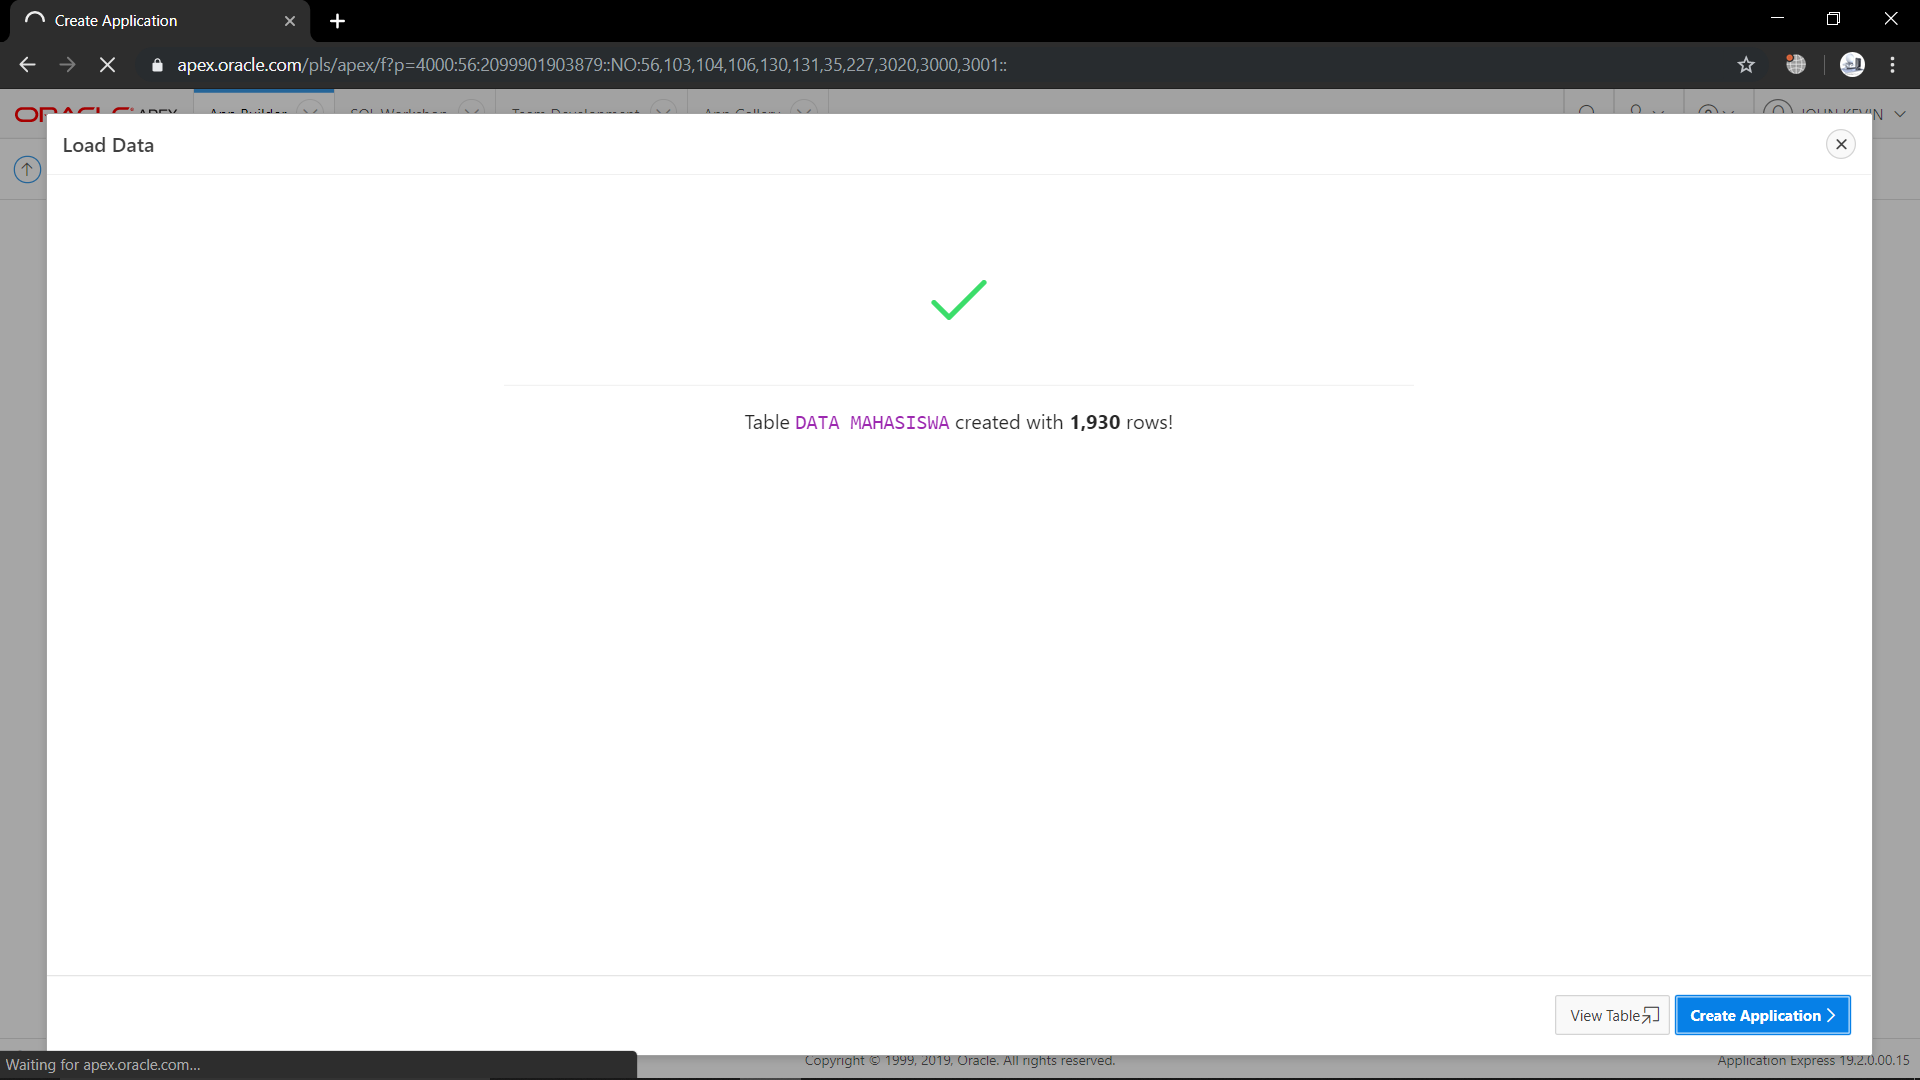
\includegraphics[width=6cm]{Figure/CA.png}
	\caption{Create}
	\label{fig:gambar}
	\end{figure}
	
	    \item Setelah dibuat, jika kalian ingin melihat aplikasi yang kalian buat tadi maka klik Run Application
    \begin{figure}[h]
	\centering
	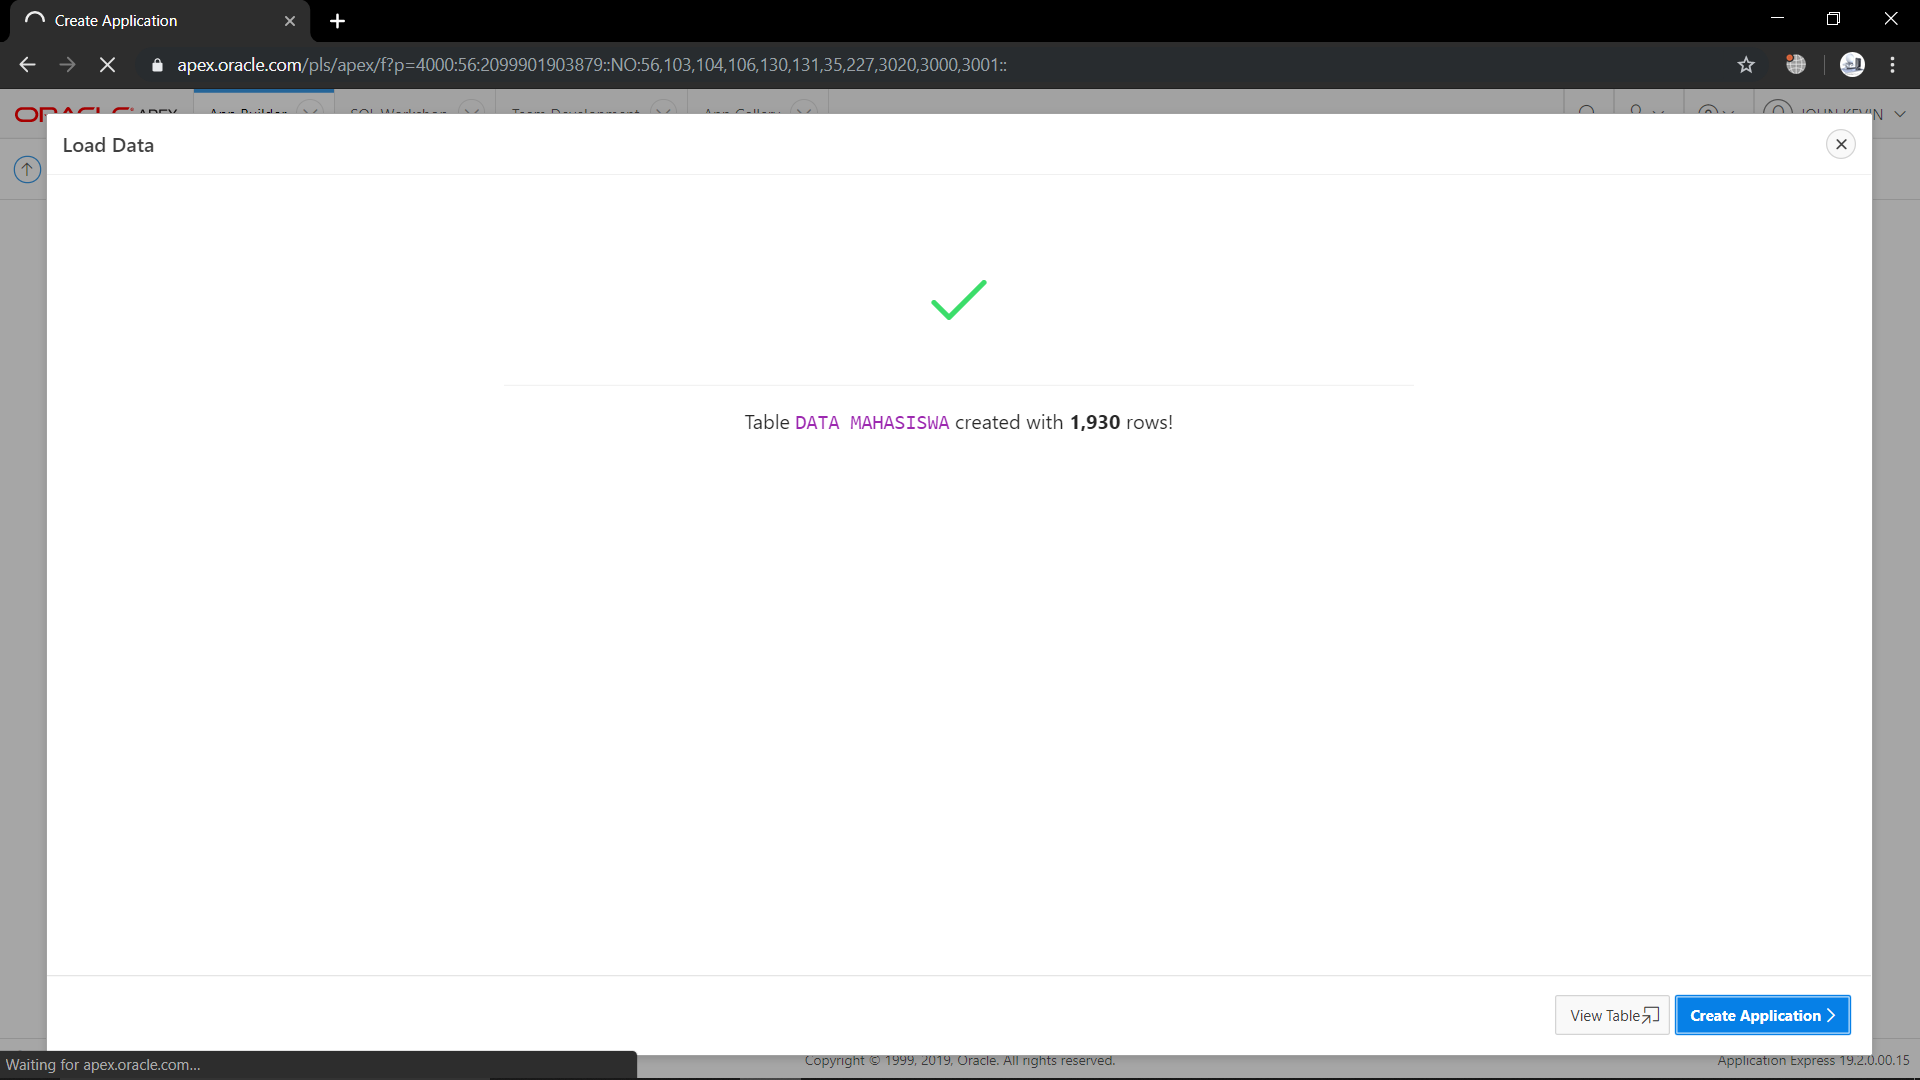
\includegraphics[width=6cm]{Figure/CA.png}
	\caption{Create}
	\label{fig:gambar}
	\end{figure}
    
    \item Sebelum masuk ke aplikasi yang telah dibuat, kalian harus login dulu terlebih dahulu memakai akun masuk oracle APEX
    \begin{figure}[h]
	\centering
	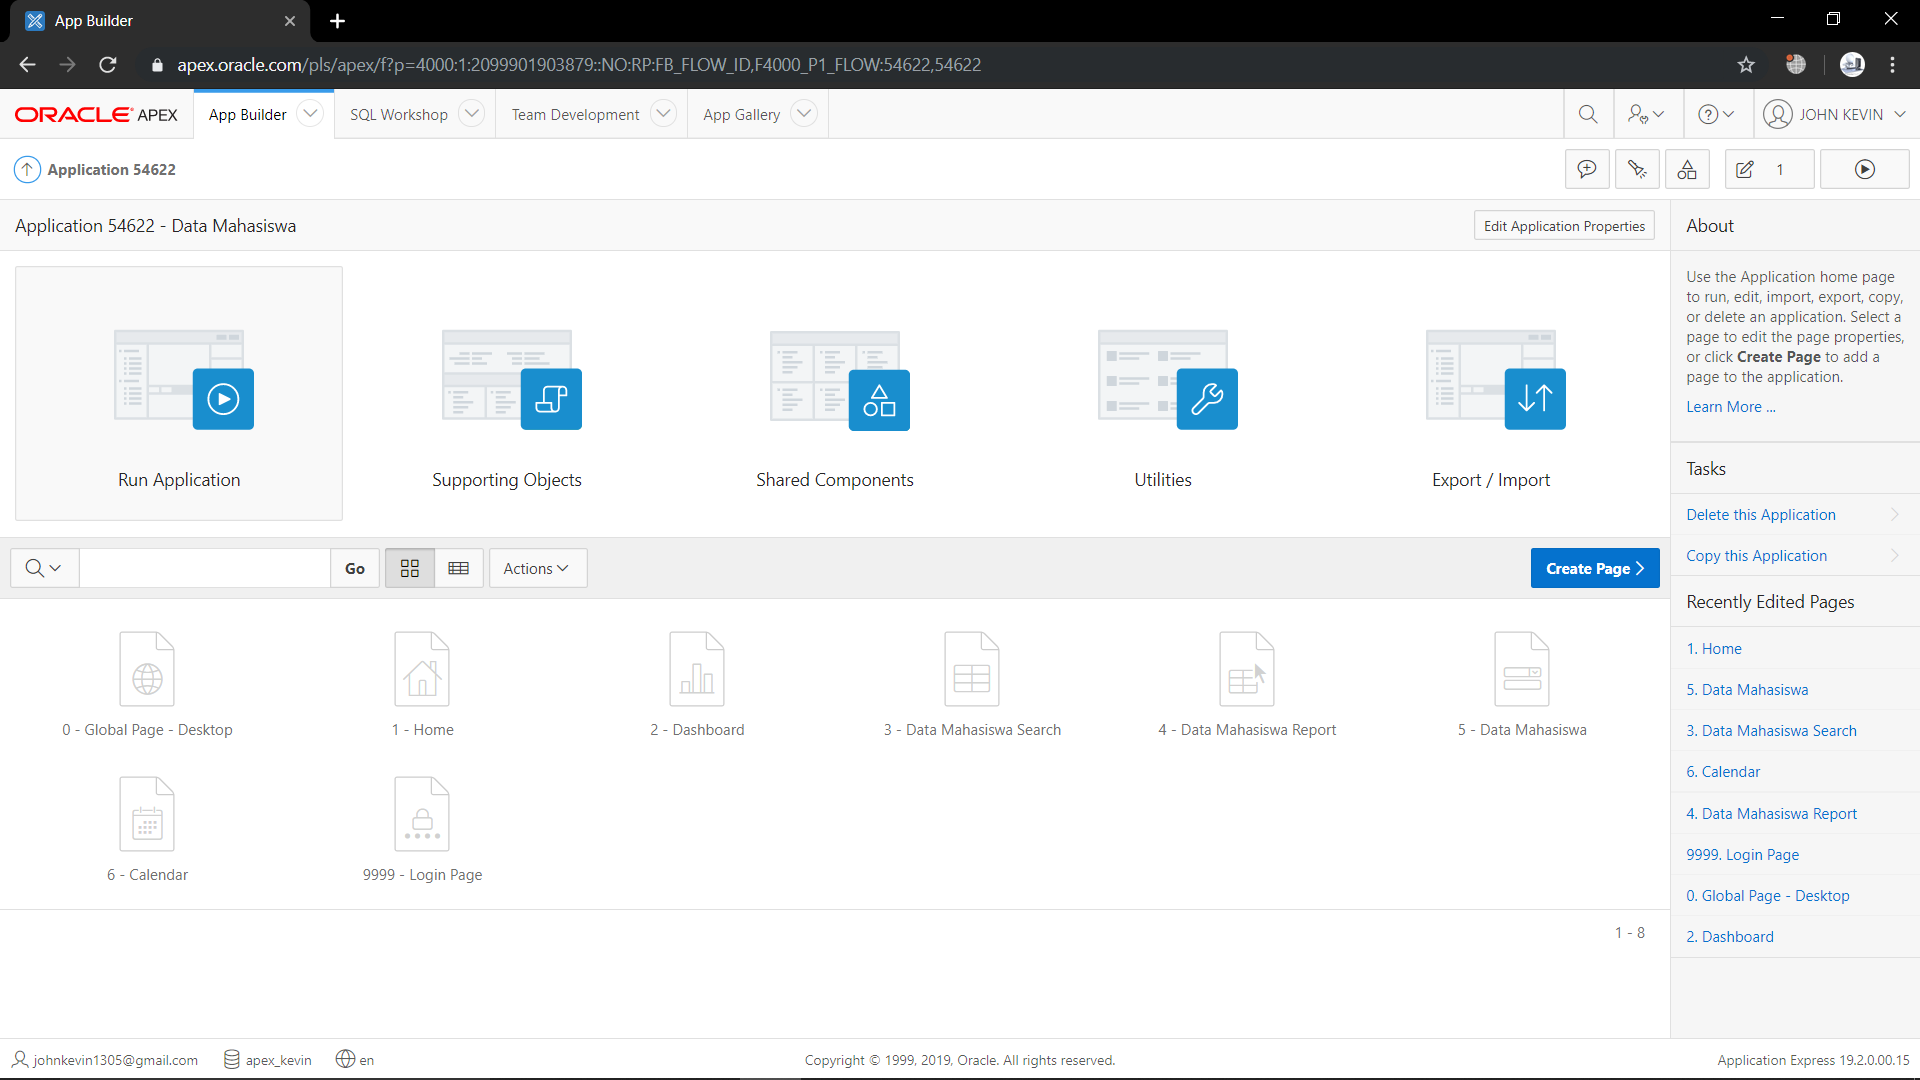
\includegraphics[width=7cm]{Figure/RA.png}
	\caption{Create}
	\label{fig:gambar}
	\end{figure}
    
    \item Setelah login maka akan masuk ke tampilan awal aplikasi yang telah dibuat
     \begin{figure}[h]
	\centering
	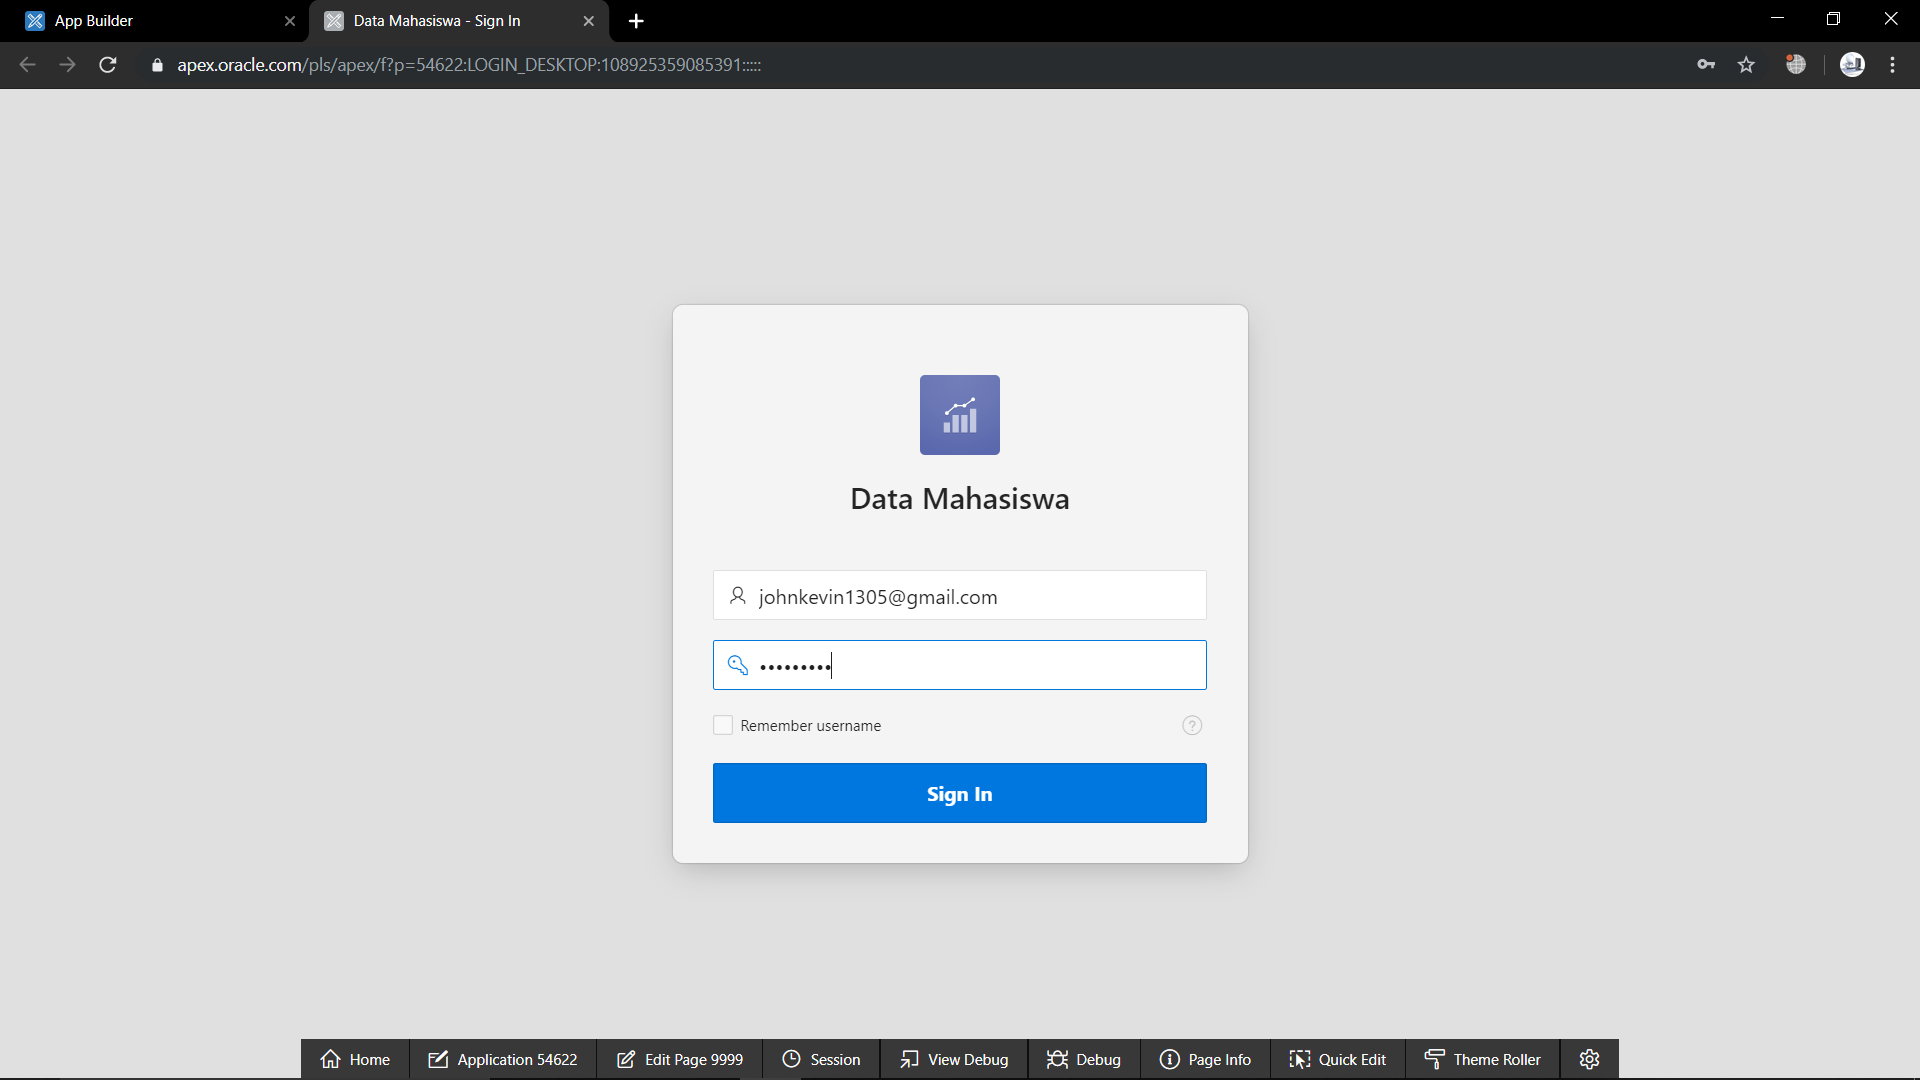
\includegraphics[width=7cm]{Figure/LRA.png}
	\caption{Create}
	\label{fig:gambar}
	\end{figure}
	
Data yang diinputkan sudah ternormalisasi, dengan menggunakan kolom yang sudah  disesuaikan dengan karakter data masing-masing. Contohnya: data nama mahasiswa, semuanya terdapat pada kolom "NAMA"
     \begin{figure}[h]
	\centering
	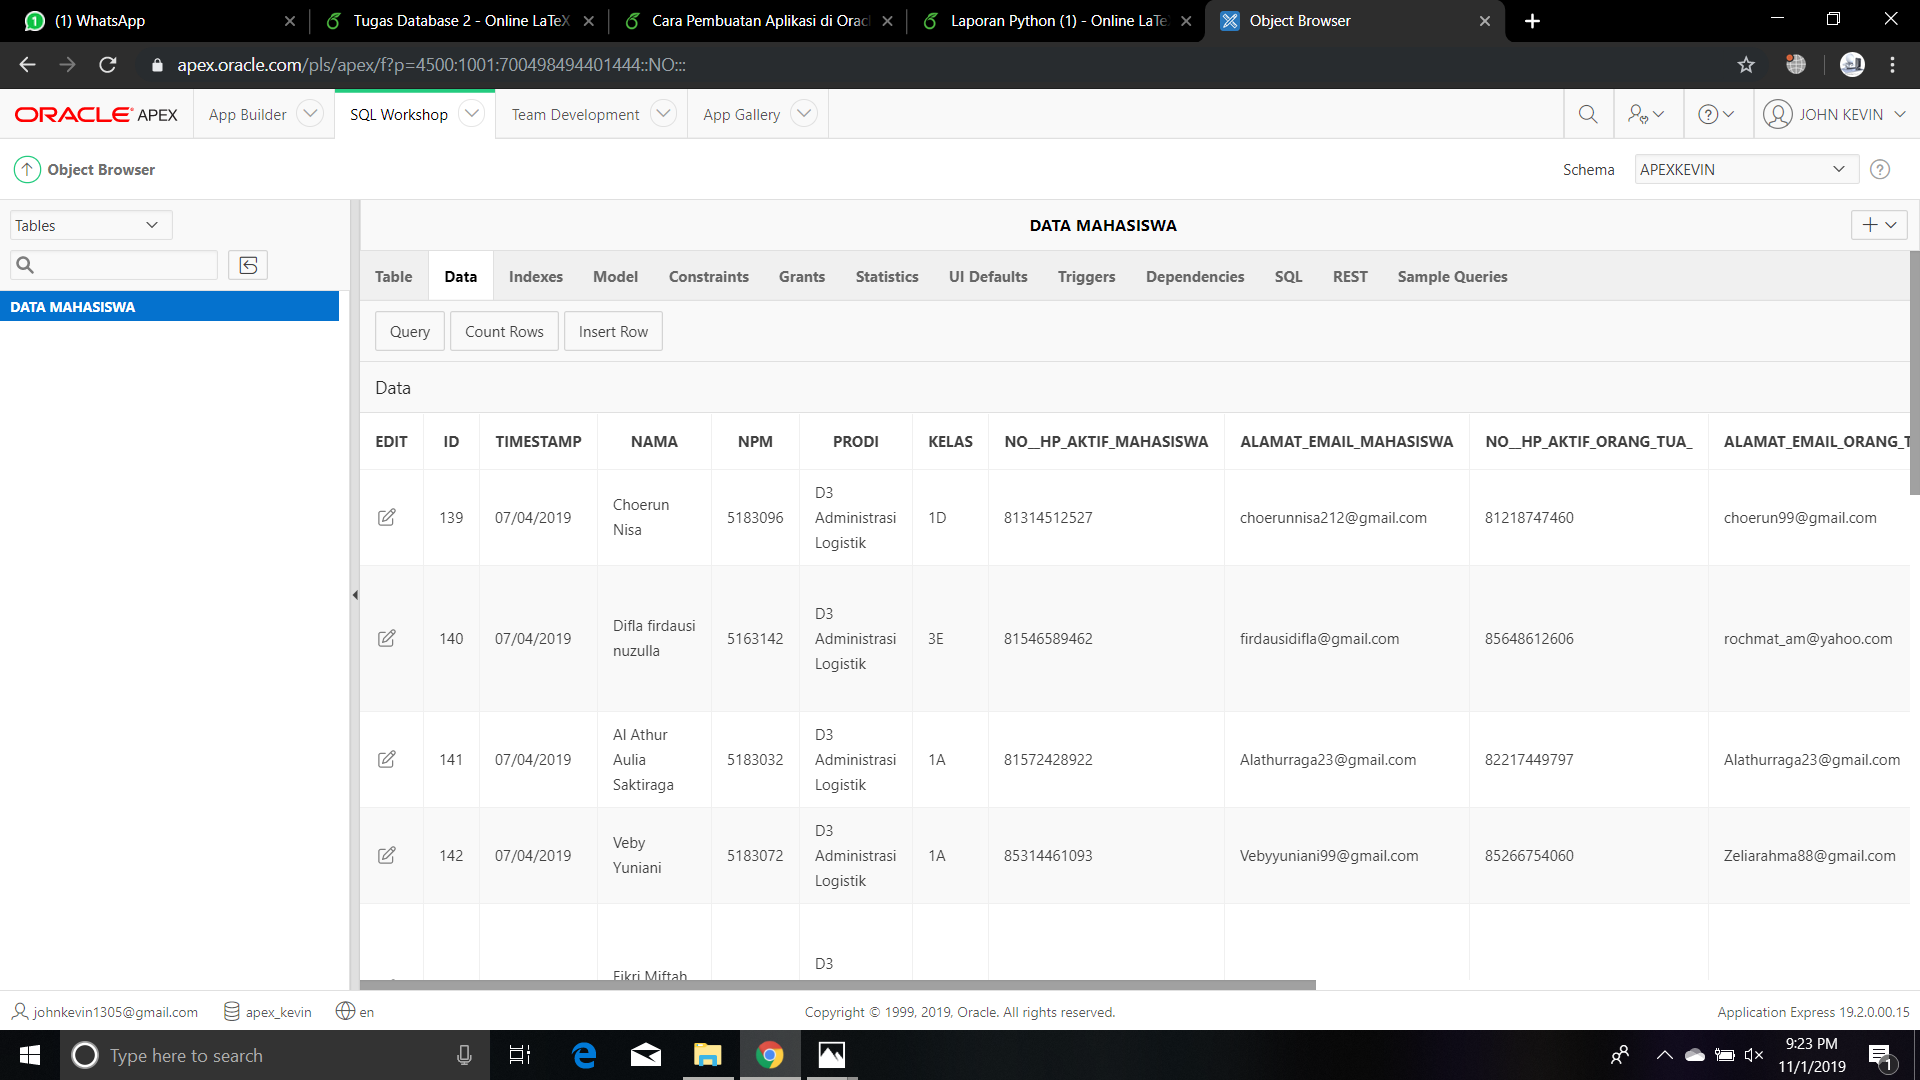
\includegraphics[width=7cm]{Figure/Norm.png}
	\caption{Create}
	\label{fig:gambar}
	\end{figure}

	
\end{enumerate}
\end{document}
